%This Thesis Template, assembled by Sam Root, is heavily based off of the one created by Chistopher Goes, available at. https://www.uidaho.edu/-/media/UIdaho-Responsive/Files/cogs/Thesis-and-Dissertation-Resources/ThesisTemplate.tex?la=en&hash=5667028A20C90A1764561B515E4BD57DE0D0D803
%I edited this one, which was designed for a Computer Science thesis, to work better for an Engineering thesis.
%Chris also credits Matthew Brown, Cara Leatherman, and Chris Zeoli

\documentclass[12pt]{UIdahoMastersThesis} %This tells the compiler to design the document based off of the file uidahomastersthesis.cls in this working directory. 
\makeatletter

\usepackage[latin1]{inputenc}
\makenoidxglossaries 

%Preamble
\usepackage{tikz} %This package allows you to make drawings - see https://www.youtube.com/watch?v=bQugbYq0BVA
\usetikzlibrary{positioning}

\graphicspath{ {./img/} } %tells the compiler to look for images in the /img folder nested in this working directory. If your \img folder is in an adjacent working directory, change it to {../img/}

\usepackage[PetersLenny]{fncychap} %This makes the chapter titles fancy: If you don't want it fancy, delete this line and uncomment the chapter title formatting under the \frontmatter below
	\ChNameVar{\LARGE\scshape}
	\ChTitleVar{\Huge\scshape}

%Make post-it notes! You can make more of these if you want different colors for different purposes
\usepackage[colorinlistoftodos,prependcaption,textsize=tiny]{todonotes}
\newcommandx{\note}[2][1=]{\todo[linecolor=orange,backgroundcolor=yellow!25,bordercolor=orange,#1]{#2}}

% --------------------------------------------------------------------------
% Thesis Information
\title{An Incredibly Cool Thesis}
\author{Joe I. Vandal}
\thesisdegree{Master of Science}
\major{Nuclear Engineering}
\advisor{Major Professor, Ph.D.}
\cmone{Committee Member, Ph.D.}
\cmtwo{Committee Member, Ph.D.}
\deptadmin{Indrajit Charit, Ph.D.}
\graddate{May, 2023}
% -------------------------------------------------------------------------

\linespread{1.3}%1.3 is on-and-a-half-spacing

% Defines section counter for front-matter. This way section number does not appear in the TOC for front-matter sections
\setcounter{secnumdepth}{0}

% Sets what level of sections show up in the table of contents. 0 = sections, 1 = subsections, 2 = sub-subsections, etc.
\setcounter{tocdepth}{1}


% Configure the PDF output (Most of this is optional, it just adds metadata to the PDF)
\hypersetup{% pdftex
pdfauthor={Joe I. Vandal},
pdftitle=PDF Title,
pdfsubject={Subject},
pdfkeywords={keywords,keyword,key,word},
pdfproducer={ShareLatex},  % e.g ShareLatex
pdfcreator={pdflatex},
pdfprintscaling={AppDefault}}

% Configure hyperlinks
\hypersetup{
	colorlinks=true, %set true if you want colored links
	linktoc=all,     %set to all if you want both sections and subsections linked
	linkcolor=black,  %choose some color if you want links to stand out
	citecolor=black,
	urlcolor=black,
}

% Changes default indenting in list of figures to 0
%\makeatletter
\renewcommand*\l@figure{\@dottedtocline{1}{0em}{2.3em}}% Default: 1.5em/2.3em
\let\l@table\l@figure
%\makeatother

% ------------------------------------------------------------
% ------------------------------------------------------------

%Adding "Eqn." before the equation number
\renewcommand{\theequation}{Eqn. \thechapter.\arabic{equation}}
%Adding new equation environment for reactions
\newcounter{chemequation}
\renewcommand{\thechemequation}{Rxn. \thechapter.\arabic{chemequation}}
\newenvironment{reaction}{%
\stepcounter{chemequation}%
\begin{equation}}%
{\tag{\thechemequation}%
\end{equation}}

% ------------------------------------------------------------
\begin{document}

\frontmatter

%\titleformat{\chapter}[block]{\scshape\LARGE}{\centering\chaptertitlename\  \thechapter:}{1ex}{\centering}{}\titlespacing{\chapter}{0pt}{-40pt}{20pt}

\titleformat{\section}[hang]{\scshape\Large}{\thesection}{1ex}{}
    \titlespacing{\section}{0pt}{0pt}{10pt}
	%\titlespacing*{\section}{0pt}{-50pt}{40pt}

\titleformat{\subsection}[hang]{\scshape\large}{\thesection}{1ex}{}
    \titlespacing{\subsection}{0pt}{0pt}{10pt}
	%\titlespacing*{\subsection}{0pt}{-50pt}{40pt}


% Head------------------------------------------------------------
% -- Title Page --
\thesistitlepage

% -- Abstract --
\frontmattersection{Abstract}
%Abstract
\begin{center}
	{\LARGE\textsc{Abstract}}
\end{center}

\lipsum[1-2]
 %Template pulls in Abstract.tex from the Preface subdirectory

% -- Acknowledgements --
 \frontmattersection{Acknowledgements}
\begin{center}
   {\LARGE\textsc{Acknowledgements}}

   This work and my coursework was completed under a Graduate Fellowship funded by \acf{nrc}. 

%Template pulls in Acknowledgements.tex from the Preface subdirectory

% -- Dedication --
 \frontmattersection{Dedication}
 \vspace*{\fill}
\begin{center}
{\LARGE\textsc{Dedication}}\vspace{0.5cm}

To my mother, Tammy, who planted and nurtured my love of science. To my father, Paul, who taught me how to design and build, and showed me that I am an engineer. To my cats, Babe and Bunyan, who stayed up with me all those late nights studying and writing. Thank you for your endless support.

\end{center}
\vspace{\fill}
%Template pulls in Dedication.tex from the Preface subdirectory

% ------------------------------------------------------------
% -- Table of Contents --
\frontmattersection{Table of Contents}
\tableofcontents
\newpage

% -- List of Tables --
\frontmattersection{List of Tables}
\listoftables
\newpage

% -- List of Figures --
 \frontmattersection{List of Figures}
 \listoffigures
 \newpage

 % -- List of Codes --
 \frontmattersection{List of Codes}
 \listof{code}{List of Codes}
 \newpage

% -- List of Acronyms --
\frontmattersection{List of Acronyms}
\printnoidxglossary
\newpage

% ------------------------------------------------------------
\mainmatter  % Starts the content part of the thesis
\setcounter{secnumdepth}{1}  % Sets depth section numbers go to.
% NOTE !! : There is a bug currently where they will not work at depth of 3, e.g section 1.2.3 will not display, but 1.2 will.

% ------------------------------------------------------------
% -- Introduction --
\chapter{Introduction}
\label{Chapter:Introduction}

\section{Background}
The \acf{msnb} is a self contained design for a liquid fueled molten salt microreactor \cite{CarterPHD,PetersonMS}. It is fueled by an inorganic form of uranium, \UF, dissolved in a coolant salt such as \flinak (a eutectic mixture of three alkali fluorides) or \flibe  (a mixture of $LiF$ and $BeF_2$) \cite{RoperOverview}. Heat is generated in the core by fission, is transported by the natural circulation of the coolant/fuel salt, and rejected to a secondary working fluid in an integrated heat exchanger. Criticality is manipulated using axial control drums, which may be rotated to aim either a neutron reflecting material or a neutron absorbing material towards the core.

\subsection{Micro Reactors}
Its like a reactor but smol. This is a test from CAES.

\subsection{Molten Salt Reactors}
\acf{lwr}


\section{Scope}
As a developing design, work has been done on neutronics \cite{PetersonMS}, thermal-hydraulics and autonomous load following \cite{CarterPHD}, and corrosion concerns \cite{RoperPHD}. However, until now, little to no work has been done on the control system. First and foremost, this work details a multiphysics characterization of the \acs{msnb} required to design a feedback controller capable of matching the core power generation to the secondary power demand. In addition to the main control mode of following power transients during normal operation, specific discussion is centered around more dynamic time periods, namely: 
\begin{enumerate*}[label=\arabic*)]
    \item initial start-up;
    \item shutdown, both planned and emergency; and
    \item restart;
\end{enumerate*}%Template pulls in Introduction.tex from the Chapters subdirectory

% -- Background --
\chapter{Background}
\label{Chapter:Background}

You're probably gonna need to do some math. You can do inline equations like $a^2+b^2=c^2$ by wrapping with dollar signs. Especially useful for inline equations is \verb=\nicefrac=, which is a package loaded, and does diagonal fractions instead of vertical. This can keep inline equations looking nice and uncramped. $K.E. = \nicefrac{mv^2}{2}.$ instead of $K.E. = \frac{1}{2}mv^2.$ You will also want separate equations like \ref{einstein}.

\begin{equation}\label{einstein}
    e=mc^2
\end{equation}

Curly braces are used in \ref{exp} for multi character sub/superscripts. It also shows how to use greek characters. There are a ton of other features for \LaTeX \; equations that you can find with Google.

\begin{equation}\label{exp}
    -1 = e^{i\pi} 
\end{equation}

Referencing equation numbers using \verb=\ref{label}= is handy because it updates the number if the numbering changes \eg you add another equations.

In addition to mathematical equations, you may also want to include chemical (\ref{rxn:methane} or nuclear (\ref{rxn:tritium}) reactions. This template has a custom environment to have a separate counter and present with a different label than mathematical expressions.

\begin{reaction}\label{rxn:methane}
    CH_4 + 2O_2 \to CO_2 + 2H_2O
\end{reaction}

\begin{reaction} \label{rxn:tritium}
    ^{6}Li + n \to {^{3}H} + \alpha
\end{reaction} %Template pulls in Background.tex from the Chapters subdirectory

% --Results and Discussion --
\chapter{Results and Analysis}
\label{Chapter:Results}

Tables and figures are handled well by \LaTeX . 

\section{Tables}

Tables can be generated using the tabular environment. To make it possible to reference them, include a caption, and automatically populate the list of tables, wrap this in the table environment.

\begin{table}[h!]
    \caption[Relevant Nuclear Constants]{Relevant nuclear constants \cite{Lamarsh}.}
    \centering\begin{tabular}{c|ccc}
                   & $\gamma \;(\%)$ & $\lambda \; (hr^{-1})$ & $\sigma \; (Mb)$ \\ \hline
        \I  & 6.39            & 0.1035                 & -                \\
        \Xe & 0.237           & 0.0753                 & 2.65
    \end{tabular}
    \label{params}
\end{table}

The caption contains two arguments. The first is wrapped in square brackets and is the "short" version that will populate in the List of Tables. The second is the "long" version, wrapped in curly braces, that will populate above the table. Table \ref{params} has 4 columns, each of which has centered data, with a vertical line after the first column. This is specified by the argument \verb={c|ccc}= after \verb=\begin{tabular}=. Columns are delimited by \& and rows are delimited by \verb=\\=. The label should come after \verb=\end{tabular}= so the compiler doesn't get confused.

\section{Figures}
The figure environment can be used to load in various images and other figures. Like with the table environment, you can develop a label to reference the figure in text, and both a short version and long version of the caption. This is handy to keep your List of Figures tidy while allowing for very descriptive captions under the figure.

\newpage

\subsection{Static Images}
These are included using the \verb=\includegraphics[options]{name}= command. There is a lot more information on the internet, including Dr. Trefor's videos. Figure \ref{BC} is an example. The argument after the \verb=\begin{figure}= is used to position the figure.

\begin{figure}[h!]
    \centering
    \includegraphics[width=0.25\textwidth]{BC}
    \caption[Big Chungus.]{A humorous image of an overweight Buggs Bunny, often referred to as `Big Chungus'.}
    \label{BC}
\end{figure}

\subsection{User Generated Drawings}

Tikz is a package that allows you to make very nice drawings right in \LaTeX \;. Dr. Trefor has a tutorial. The learning curve is steep, and honestly is more difficult to use than GUI sandbox based drawing application, but it has the benefit of being able to keep typeface formatting very consistent. See how nice the equations look in Figure \ref{strip}? Try doing that in MS Paint. 

\begin{figure}[h!]\centering
    

\begin{tikzpicture}
\draw[green, very thick] (-1,-1) rectangle (1,1);
\filldraw[green!10] (-1,-1) rectangle (1,1);
%Bottom
\draw[->] (0,-2)--(0,-1);
\draw node at (-0.15,-2.15) {\small{$c_{He}^{in} = 0$}};
%Top
\draw[->] (0,1)--(0,2);
\draw node at (0.15,2.15) {\small{$c_{He}^{out} = \nicefrac{c_{salt}^{out}}{H^*}$}};
%Left
\draw[->] (-2.75,0)--(-1,0);
\draw node at (-1.0,0.5) [anchor=east]{\small{$c_{salt}^{in} = Xe(t)$}} ;
%Right
\draw[->] (1,0)--(4,0);
\draw node at (1.0,0.5) [anchor = west]{\small{$c_{salt}^{out} = c_{salt}^{in}-c_{He}^{out}\frac{\dot{V}_{He}}{\dot{V}_{salt}}$}};
\end{tikzpicture}

    \caption{Schematic Drawing of Xenon Stripping Module} 
    \label{strip}
\end{figure}

\newpage
\subsection{Animations}
The graphicx package cannot accept .gif files, so the animate package can be used as a proxy. You will need each frame to be an individual .png, but this allows you to stack images over one another, which can give a time component to 2-D plots, or allow you to look at multiple planes of a drawing in a single figure. You will need to open the file in a proper PDF viewer like Adobe - web browsers and PDF previewers found in Overleaf, Atom, VSCode, etc. cannot handle this powerful functionality. I'm not sure if this functionality is allowed in the actual thesis submission, but it can be useful in presentations or meetings. Figure \ref{Bateman} is a visualization of the Bateman equations  causing the xenon spike following the shutdown of a nuclear reactor. It loops through bar-200 to bar-248 at 2 frames per second. You can also step through frame by frame using the arrow controls. Note that feature can cause compile times to be very long so you may wish to comment it out. 

\begin{figure}[h!]
    \centering
    \animategraphics[width=0.60\textwidth, controls]{2}{scram/bar-}{200}{248}
    \caption{Nuclide Concentration Rates of Change - Reactor Scram}
    \label{Bateman}
\end{figure} %Template pulls in Results.tex from the Chapters subdirectory

% -- Conclusions --
\chapter{Conclusions}
\label{Chapter:Conclusions}

\section{Limitations}

\section{Future Work}

\section{Summary Remarks} %Template pulls in Conclusions.tex from the Chapters subdirectory

% ------------------------------------------------------------
% -- References -- 

\clearpage
\renewcommand\bibname{References}
\addcontentsline{toc}{chapter}{\textsc{\bibname}}%Changes 'Bibliography' to 'References' per UIdaho Thesis styling requirements
\bibliographystyle{nsf} %Uses nsf.bst for formatting
\bibliography{References.bib} %Tells BibTex to look for sources in the file in the braces.

% ------------------------------------------------------------
% -- Appendices --
\clearpage 
\appendix % Marks start of appendices

%Test
\chapter{Codes}
You may have done some coding in your thesis. You can share it with the verbatim package, but it looks a lot nicer to have a specific environment for code blocks. You can even include language specific syntax highlighting. The style file mypythonhighlight.sty in the working directory is set up for python, but you can find packages for other languages too!. I made a custom code environment which gives you a caption over the code block and lists it automatically in the List of Codes. 

The simplest way to include code is to type it directly in the .tex file in the \verb=\begin{python}= environment defined by the .sty file. Just like with figures, tables, and equations, you can label and reference them. Just like with the verbatim environment, indentation is preserved, as displayed by the (useless) example, Code \ref{code:hello}

\begin{code}\caption{Hello!} \begin{python}
    print("Hello World") #comment
    try:
        a=2/x
    except ZeroDivisionError:
        print('undefined')
\end{python}\label{code:hello}\end{code}

You might be discussing a single aspect of your code in the body of your thesis. Inline codes like \pyth{import numpy} are very useful for doing this, distinguishing the commands from regular text by using the code font and syntax coloring.

My preferred way of including codes in the document is by using the custom \verb=\inputpython= command. Code \ref{code:fstrings} displays lines 1 to 3 of test.py, located in the py subdirectory. It's an example of a very nice python feature, fstrings. 

\begin{code}\caption{F strings}
\inputpython{py/test.py}{1}{3}
\label{code:fstrings}\end{code}

You can customize the syntax highlighting by digging into mypythonhighlight.sty. This may be nice if you are using a specific library and want the keywords in that library to be highlighted as keywords, but the .sty file doesn't identify them as keywords by default.%Template pulls in Codes.tex from the Appendix subdirectory

\end{document}

% ** DO NOT PUT ANYTHING AFTER THE END OF THE DOCUMENT! **
